% enaR: Tools for Ecosystem Network Analysis
% Target: Methods in Ecology and Evolution
% February 2014
% ---------------------------------------------------
\documentclass[11pt]{article}
\usepackage[super, sort]{natbib}
  \bibpunct{(}{)}{;}{a}{,}{,} % required for natbib
\bibliographystyle{mee}

\usepackage[margin=1in]{geometry}

\usepackage{amsmath,amssymb,amsthm,amsfonts}
\usepackage[]{graphicx}
\usepackage{setspace}
\usepackage{lineno} %numbers lines
\usepackage{qtree} %draw tree structures
\usepackage{url}

% --- SRB Defined functions ----
\newcommand{\ppr}{\lambda_1(\mathbf{A})}
\newcommand{\ID}{I/D}
\newcommand{\g}{\lambda_1(\mathbf{G})}
\DeclareMathOperator{\diag}{diag}
\def\citeapos#1{\citeauthor{#1}'s (\citeyear{#1})}
\newcommand{\R}{R}
%\newcommand{\S}{S}
\newcommand{\enaR}{\texttt{enaR}}
\newcommand{\vnorm}[1]{\left|\left|#1\right|\right|}
\newcommand{\midtilde}{\raisebox{-0.25\baselineskip}{\textasciitilde}}
\def\tableline{\vskip .1in \hrule height 0.6pt \vskip 0.1in}
% ----------------
\usepackage[ pdfauthor={Stuart R. Borrett},
pdfkeywords={ecological network analysis, network environ analysis},
pdfpagemode=UseOutlines, bookmarks=T, colorlinks,
linkcolor=blue,citecolor=blue, pdfstartview=FitH,
urlcolor=red]{hyperref}

% ---- FRONT MATTER -----

\title{\enaR: An \R\ package for Ecosystem Network Analysis}
\author{Stuart R. Borrett$^{a,*}$ and Matthew K. Lau$^b$
  \\ {\footnotesize $^a$ Department of Biology and Marine Biology,} \\
    {\footnotesize University of North Carolina Wilmington, Wilmington, NC, 28403}
  \\ {\footnotesize $^b$ Department of Biological Sciences and the
    Merriam-Powell Center for Environmental Research,} \\
{\footnotesize Northern Arizona University, 617 S.\ Beaver St., Flagstaff, AZ, 86011}
  \\ {\footnotesize $^*$ Corresponding author, borretts@uncw.edu} }

% ------------------------
\begin{document}

%%%%%%%%%%%%%%%%%
%%%Title Page
%%%%%%%%%

\begin{description}
  \item[\textbf{Title}:] \enaR: An \R\ package for Ecosystem Network Analysis
  \item[\textbf{Running Title}:] R ecosystem network analysis package
  \item[\textbf{Word Count}:] 3110
  \item[\textbf{Authors}:] Stuart R. Borrett, Matthew K. Lau
  \item[\textbf{Addresses}:] \
    \begin{itemize}
    \item SRB: Department of Biology and Marine Biology, University of
      North Carolina Wilmington, Wilmington, NC, 28403
    \item MKL: Department of Biological Sciences and the
      Merriam-Powell Center for Environmental Research, Northern
      Arizona University, 617 S. Beaver St., Flagstaff, AZ, 86011
    \end{itemize}
  \item[\textbf{Contact Details}:] \
    \begin{itemize}
    \item Email: borretts@uncw.edu
    \item Phone: 910.962.2411
    \item Fax: 910.962.4066
    \end{itemize}
\end{description}

\pagebreak

\maketitle

\begin{spacing}{2}
\linenumbers

\tableline
\section*{Abstract}
\begin{itemize}
\item Network analysis is a useful approach for complex, relational
  datasets in many biological fields, including ecology and molecular
  and evolutionary biology.
\item Here, we introduce \enaR , an \R\ package for conducting
  Ecosystem Network Analysis (ENA), an analytical tool set rooted in
  ecosystem ecology with over 30 years of development, which examines
  the structure and dynamics of matter and energy movement between
  discrete ecological compartments (e.g., a food web).
\item In addition to describing the primary functionality of the
  package, we also highlight several value added features, including a
  library of 100 empirical ecosystem models, the ability to analyze
  and compare multiple models simultaneously, and connections to
  useful ecological network analysis tools in \R .
\end{itemize}

KEYWORDS: network analysis, ecosystem, open-source software, network
environ analysis, ascendency, input--output analysis, food web, urban
metabolism, Ecopath, WAND \tableline

\section{Introduction}
% Network Ecology & its significance
Network Ecology -- the study of ecological systems using network
models and analyses to characterize their structure, function, and
evolution -- is a large and rapidly growing area of ecology
\citep{proulx05}. %, borrett12_netecol}.
For example, \citet{ings2009} discovered that a notable fraction of
2008 publications in 11 select journals were related to food webs
($\approx$2.4\%), mutualistic networks ($\approx$0.9\%), and
host-parasitoid networks ($\approx$0.06\%). Likewise,
\citet{borrett14_rise} found that the percent of ecology and
evolutionary biology papers indexed by Web of Science that could be
classified as Network Ecology increased from 1.3\% in 1991 to more
than 5\% in 2012.  This rise of Network Ecology contributes to,
mirrors, and builds on the more general growth of network sciences
\citep{wasserman94, barabasi12, borgatti2003network,
  freeman2004development, newman03review}.

%% However, it seems likely
%% that the field is growing in part because the network approach is
%% useful.
%; it enables scientists address fundamental ecological
%questions.

% ENA & Questions ---
Ecosystem Network Analysis (ENA) is a branch of Network Ecology that
has been used to address a range of key ecosystem questions
\citep{borrett12_netecol, fath99_review, ulanowicz86}.
%As many ecosystem questions center on how species are connected across
%a web of energy and matter transactions, Ecosystem Network Analysis
%\citep[ENA; ][]{ulanowicz86,fath99_review} has helped address a range
%of key questions.
For example, in the food web of Big Cypress National Preserve
(Florida, USA) \citet{bondavalli99} found evidence of an indirect
mutualism between the American alligator and some of its prey
items. Applications of ENA have also lead to new insights into the
classic trophic questions of ``What limits food-chain length?''
\citep{ulanowicz2014} and ``Are food webs modular?''  \citep{krause04,
  allesina05_scc, borrett07_jtb}.  \citet{hines12} used ENA to
quantify the relative importance of coupling between biogeochemical
processes (e.g., nitrification) in the Cape Fear River estuary
sedimentary nitrogen cycle.  Further, scientists have used ENA to
investigate differences in urban sustainability \citep{bodini02,
  zhang10_ecomod, chen12, bodini2012cities}.  Collectively, this work
consistently shows the power of a transactional network to generate
unexpected ecological relationships that then influence the system
function and evolution \citep{ulanowicz97, patten91,
  jorgensen07_newecology}.

% what is ENA
% Ecosystem Network Analysis (ENA) is a branch of Network Ecology
% \citep{ulanowicz86, fath99_review, borrett12_netecol} that ecologists
% have used to investigate the form and function of organism
% connectivity across the intricate web of interactions that comprise
% the ecosystem.
% % Examples of Applications and Questions
% %% PICK UP HERE
% Food webs provide an iconic example of this is a food-web built by tracing the energy or
% nutrients through the system.  However, the techniques have been used
% in multiple ways.  For example, \citet{patten82} used a storage-based
% ENA to identify two nearly separate hydrologic subsystems in the
% Okefenokee Swamp, USA.  \citet{bondavalli99} used a Mixed Trophic
% Impacts ENA to discover that in the Florida Everglades the American
% alligator is an indirect mutualist with several of its prey, including
% frogs, and \citet{hines12} used a flow-based and environ ENA to
% quantify the coupling between biogeochemical processes (e.g.,
% nitrification + anammox) in the Cape Fear River estuary sediment
% nitrogen cycle.

% Software Objectives
\enaR\ is an open-source software to facilitate ENA.  Extant ENA
software \citep{ulanowicz91, kazanci07, allesina04_wand,
  christensen04, fath06} each have critical limitations, which led us
to three primary design objectives for \enaR .
The first objective was to collect the major ENA functions into a
single software package.  While multiple investigators have
contributed to algorithmic development \citep[e.g.,][]{finn76,
  ulanowicz86, ulanowicz91, fath99_review, allesina03}, the broad set
of tools is not available in a single existing software.  The second
objective was to increase the availability and extensibility of the
software. We chose to use \R\ in part because of its
increasing popularity as an analytical tool in the biological sciences
\citep[e.g.,][]{dixon2003vegan, metcalf2012, revell2012phytools}.
Further, users can freely download a stable version of the package
from the CRAN website
(\url{http://cran.r-project.org/web/packages/enaR/}), and the code for
every function in \R\ is available from within \R\ (e.g.,
\texttt{edit($function\_name$)}).  In addition, \enaR\ development is being managed
via GitHub (\url{https://github.com/TheSeeLab/enaR}) to encourage
collaborative development.  The third design objective was to enable
\enaR\ users access to network analysis tools from other
disciplines.  To enable this, \enaR\ was designed to work directly
with two existing \R\ network analysis packages:  \texttt{network}
\citep{butts08_network} and \texttt{sna} \citep{butts08_social}.  In
summary, the aim of the \enaR\ package is to make ENA tools more
available and easier to use, adapt, and extend.
% does this sufficiently address the editors concerns about "novelty".

% Paper Objectives
In this paper, we present an overview of \enaR\ and highlight some of
its functionality.  A full description of the ENA algorithms and their
use and interpretation is beyond the scope of this short paper, but we
refer interested readers to a selection of reviews as an entry point
to ENA \citep{fath99_review, ulanowicz97, fath06, schramski11,
  jorgensen07_newecology}.  For a more comprehensive description on
how to use the \enaR\ package, please refer to the package vignette:
\url{http://cran.r-project.org/web/packages/enaR/vignettes/enaR.pdf}.
% part of what we need to do is communicate to the editor the shear
% size of the package and its capability.

\section{Overview of \enaR}
ENA is an agglomeration of algorithms developed to analyze network
models of energy or matter movement in ecosystems
\citep[e.g.,][]{hannon73, fath99_review, ulanowicz86}, but it can
generally be applied to any Input-Output system that follows a
thermodynamically conserved unit among the compartments.  Thus, it is a
family of related algorithms to analyze the ecosystem from several
perspectives including its structure, flow, storage, and utility.
Together, these analyses function as a ``macroscope'' to investigate
(1) whole system organization, (2) the direct and indirect effects
among system components, and (3) the processes that create and sustain
ecological systems.
% Table~\ref{tab:alg}
%describes the the main analyses in the package. \enaR\ also includes a
%number of functions to assist with data import, manipulation, and
%export, as well as some specialty analyses (Table~\ref{tab:alg2}).
In this section we provide an overview of these algorithms and tools
include in the \enaR\ software.  After describing the required model
information, we highlight the primary ENA algorithms included in
\enaR .  We then walk through an example application of the \enaR\ Flow
analysis.

\subsection{Data Requirements and Input}
% ENA Data requirements and Input -- no math
ENA is a data-intensive methodology.  The system is modeled as a set
of compartments or network nodes that represent species,
species-complexes (i.e., trophic guilds or functional groups), or
non-living components of the system in which energy or matter is
stored.  These nodes are connected by a set of direct energy or matter
transactions among the nodes, termed directed edges or links.  These
models also have energy--matter inputs into the system and output
losses from the system.  In summary, the full set of data required includes:
(1) internal flows, (2) boundary inputs, (3) boundary exports, (4)
boundary respiration, (5) boundary outputs, which may be the sum of
exports and respiration, (6) biomass or storage values, and (7)
designation of living status of each node.  While all seven elements
are required for a full analysis, the specific data requirements
varies among the ENA algorithms.

The primary ENA algorithms in \enaR\ assume the model data is
presented as an \R\ network data object defined in the
\texttt{network} package.  Given the data elements, users can use
the \texttt{pack} function to combine the data elements into the \R\
network data object. While a standard data format for an ENA model
does not yet exist, there are two commonly used formats.  First, there
is the Scientific Committee for Ocean Research (SCOR) format that is
the required input to NETWRK \citep{ulanowicz91}, and the second
format is the Excel sheet formatted data that is the input to WAND
\citep{allesina04_wand}.  The \enaR\ package includes a
\texttt{read.scor} and a \texttt{read.wand} function to read in these
common data formats (Table~\ref{tab:algIO}).

\subsection{Visualization}
% Visualization
Visualization of network models can be an essential analytical tool
\citep{moody05dynamic, lima2011visual}.  Because \enaR\ is built
specifically to use the \texttt{network} package and data type, it is possible to
quickly create network plots of the model internal structure.
Fig.~\ref{fig:example}a shows an example visualization of
\citeapos{dame81} Oyster Reef ecosystem model.  The \texttt{network}
package includes three network layout algorithms: circle,
Fruchterman-Reingold, and Kamada-Kawai.  The Fruchterman-Reingold
algorithm used here is the default.  The \R\ script to generate this
visualization is included in the online supplementary information.

\subsection{Algorithm Overview}
% enaR Algorithms
\enaR\ includes many of the most commonly used ENA algorithms
(Table~\ref{tab:alg}), along with a number of work flow tools and specialty
analyses (Tables~\ref{tab:algIO} and \ref{tab:algaux}).  Note that the nine
primary ENA functions begin with the prefix `ena' followed by the
specific analysis name (see Table~\ref{tab:alg}).  There are a total
of 34 functions in the \enaR\ package.

\citet{scharler09comparing} identify two schools of ENA.  The first
school is based on the work of Robert Ulanowicz and colleagues at the
University of Maryland \citep{ulanowicz86, ulanowicz97,
  ulanowicz09_window}.  Primarily focused on trophic ecology, this
approach uses information theory and the ascendency concept that
characterizes ecosystem growth and development \citet{ulanowicz86,
  ulanowicz97}.  This work is often referred to as ``Ecological
Network Analysis'' as it predates many other types of network ecology.
The second school is based on the work of Bernard Patten at the
University of Georgia \citep{patten76, matis81, patten82,
  fath99_review}.  Steeped in dynamic equations, simulations, and
systems analysis, this approach developed around the environ concept
that formalizes the concept of environment \citep{patten78}, and has
often been referred to as ``Network Environ Analysis.''
\enaR\ currently captures all of the Patten School algorithms
previously implemented in NEA.m \citep{fath06}.  Presently, the
Ulanowicz School algorithms are more limited, including the ascendency
calculations \citep{ulanowicz97} and mixed trophic impacts analyses
\citep{ulanowicz90}; however, we expect the package capabilities to
continue to grow, especially with the assistance of new users.  This
combination of the Patten and Ulanowicz schools of analyses is rare in
extant software.

\subsection{Example Application}
% Apply enaR to a single model.
Given a network model, applying ENA algorithms with \enaR\ is straight
forward. We demonstrate how to use the package with an example Flow
analysis on \citeapos{dame81} model of energy flow in an Oyster Reef
ecosystem. Table~\ref{tab:flow} shows the example script.  The
analysis involves: (1) loading the model data, (2) checking and
balancing the model if necessary, and (3) inputing the balanced model
into the analysis function.  The final step is interpreting the
analytical output. This is a typical workflow for ENA.

After loading the \enaR\ package, the next step is to enter the model
data.
%In this example, we use the \texttt{read.scor} function to
%import the SCOR formatted data from a text file, which is assumed to
%be in the current \R\ working directory (online supplement).
Here, we have extracted the model information from the paper and
created a vector of node names, the flow matrix (F), inputs (z),
outputs (y), and the logical vector indicating whether or not the
nodes are living (Table~\ref{tab:flow}).  We then use the
\texttt{pack} function to create the required network data object.
The next step is to apply the \texttt{ssCheck} function ensure that
the model is at steady-state, which is one of the assumptions of the
flow analysis \citep{finn76, fath06}.  If the model had not been at
steady-state, we could have then applied one of four automated
balancing algorithms \citep[AVG, Input-Output, Output-Input,
AVG2;][]{allesina03} to force the model into a steady-state.  We then
apply the \texttt{enaFlow} function to the model to perform the
desired ENA flow analysis.  As shown with the \texttt{attributes}
function, this analysis returns 4 matrices ($\mathbf{G}$,
$\mathbf{GP}$, $\mathbf{N}$, $\mathbf{NP}$) and two vectors
(throughflow, $T$, and a vector of 20 whole-network statistics, $ns$).

Interpreting the ENA results is the final challenge.  Here, we provide
a few illustrative interpretations of the Flow analysis.  Starting
with the whole-network flow statistics, we see that the total system
throughflow (TST) of the oyster reef model is 83.6 Kcal m$^{-2}$
d$^{-1}$. TST is a measure of the total activity of the system, which
is often referred to as the size or power of the system.  The Finn
Cycling Index (FCI) indicates that 11\% of this activity was generated
by recycling.  Further, the average path length (APL = 2.02) shows
that an average input passes over two paths before exiting the system,
and the ratio of indirect to direct flows (ID.F = 1.58) indicates that
the indirect flow exceeds the direct flow in this system.  Together,
these whole network indicators show the importance of indirect
interactions in the system.  A next analytical step might be to apply
the Utility or Mixed Trophic Impacts analyses to determine the net
relationships among the ecosystem components when we consider the
direct and indirect interactions, but this is beyond our analysis here.
% Patten (1991) showed that ....
More detailed guidance for how to interpret ENA results can be found
in previously published literature \citep{fath06, schramski11,
  jorgensen07_newecology}.


%%%%%%%%%%%%%%%%%%%%%%%%%%%%%%%%%%%%%%%%%%%%%%%%%%%%%%%%%%%%%%%%%%%%%%%%%%%%%%%%%%
\section{Value Added Features}
There are several features of the \enaR\ package beyond the core
analyses that add substantive value for users.  In this section, we
highlight several value added features, including a library of 100
ecosystem network models, methods for conducting batch analysis (i.e.,
simultaneous analysis of multiple models), and connections to other
analytical software.

\subsection{Model Library}
% Model Library
To facilitate new systems ecology and network science, we included a
library of 100 previously published ecosystem network models with the
\enaR\ package. These models each trace a thermodynamically conserved
unit (e.g., C, N, P) through a particular ecosystem.  The models in
this set are empirically-based in that the authors attempted to model
a specific system and parameterized the model to some degree with
empirical estimates.  While the library includes models used previously to
test several systems ecology hypotheses \citep{borrett10_idd,
  borrett10_hmg, salas11_did, borrett13}, and the set has a 47\%
overlap with the set of models previously collected by Dr.\ Ulanowicz
(\url{http://www.cbl.umces.edu/~ulan/ntwk/network.html}), the full
set has not previously been collected and distributed together.

We have tentatively split these models into two classes.  The most
abundant class is the trophic network models. % (Table~\ref{tab:TRO}).
These models tend to have a food web at their core, but also include
non-trophic fluxes generated by processes like death and excretion.
The annual carbon flux model for the mesohaline region of the
Chesapeake Bay is a typical example \citep{baird89}.  The second class
of models focuses on biogeochemical cycling.  % (Table~\ref{tab:BGC}).
In contrast to the trophic networks, the biogeochemical cycling models
tend to have more highly aggregated nodes (more species grouped into a
compartment), include more abiotic nodes that could represent chemical
species (e.g., ammonia in a nitrogen cycle), have a lower dissipation
rate, and therefore they tend to have more recycling
\citep{christian96, borrett10_idd}.  \citeapos{christian03} models of
nitrogen cycling in the Neuse River Estuary are good examples of the
class.  The package vignette has a full listing of the models included
along with references to their original publications \citep{enar}.
% maybe include Amelia's map

\subsection{Batch Analysis}
Advances in ecosystem ecology have been made by comparing network
metrics across multiple ecosystem models. For example,
\citet{christensen95} applied ENA to identify and compare the maturity
of 41 ecosystem models, and \citet{vanoevelen2011canyon} compared the
the organic matter processing of food webs in three sections of the
Nazar{\'e} submarine canyon.  The \enaR\ tool simplifies the work flow
for these types of comparison. Given a list of models like the model
library, it is possible to quickly analyze multiple models using R's
\texttt{lapply} function (see \texttt{help}(``lapply'')).  This
facilitates the kind of comparative network analysis often of interest
to ecologists \citep{monaco97,christian05_cnea, whipple07}.
% I could use examples from ECOMOD special issue.

Batch analysis can be used in several additional ways.  One
application is for meta-analyses, such as tests of the generality of
hypothesized ecosystem properties like network non-locality
\citep{salas11_did}, %and network homogenization
                     %\citep{borrett10_hmg},
or to investigate how physical features might influence ENA results
\citep{niquil2012physical}. Fig.~\ref{fig:example}b illustrates the
rank-ordered network homogenization statistic for the 56 trophic-based
ecosystem models in the library. Notice that the homogenization
statistic is greater than one in all of these models indicating that
the network of indirect interactions tend to more uniformly distribute
the resources than is obvious from the direct interactions, which
extends previous results of \citet{borrett10_hmg} to include several
new models.  A second kind of application is the exploration of new
ENA inter-relationships.  With the collection of algorithms and the
library of models, we can now investigate possible relationships among
ENA indicators from different schools (Fig.~\ref{fig:example}c). The
\R\ script to generate Fig.~\ref{fig:example} is available as an
online enhancment.  A third application of batch analysis is to
investigate the previously unknown empirical ranges of ENA
whole-network statistics, which may be useful for interpreting results
from specific applications.  Fig.~\ref{fig:ns} shows the observed
distribution of values for selected network statistics from the 100
models in the library easily analyzed using \texttt{lapply} and the
associated \enaR\ functions.


\subsection{New Connections}
% Connections to other tools (SNA, igraph)
A third added benefit of the \enaR\ package design is that it enables
network ecologists easier access to other network tools and analyses
that might be useful.  The \enaR\ package uses the \R\ network data
structure defined in the \texttt{network} package
\citep{butts08_network}.  This means that network ecologists using \enaR\
can also use the network manipulation functions and visualization
features of the \texttt{network} package. Further, the \R\ Social
Network Analysis (SNA) package, \texttt{sna}, \citep{butts08_social} also uses this
network data object.  This means that network ecologists can apply
many of the SNA algorithms directly to their ecological network
models.  Fig.~\ref{fig:example}d illustrates applying the betweenness
centrality function to the Chesapeake Bay trophic model
\citep{baird89} and visualizing the results using a target
centrality plot \citep{brandes03}.  This analysis highlights the
central role of Sedimentary Particulate Carbon and bacteria in the
Sediment Particulate Organic Carbon (POC) in the carbon flux of the
estuary.

In addition, \enaR\ can be a starting point for ecosystem network
ecologists to use other \R\ network tools.  For example, the
\texttt{iGraph} package provides functions to apply classic graph
theory \citep{csardi06}.  The \texttt{limSolve} package provides
capabilities to infer network model fluxes from empirical data by
linear inverse modeling \citep{soetaert09}, which can also be used for
uncertainty analyses of ENA \citep{kones09}. There are a wealth of
additional \R\ package that network ecologists may find useful
including \texttt{bipartite} \citep{dormann2008}, \texttt{vegan}
\citep{dixon2003vegan}, \texttt{Cheddar}
\citep{hudson2013}, and packages in the \texttt{statnet} family
\citep{handcock2008statnet}.

\section{Conclusion and Future Development}
% Existing Software/Tools : NETWRK, WAND, ECOPATH, NEA.m EcoNet
% The first widely distributed
% tool for ENA was NETWRK \citep{ulanowicz91}, a collection of analyses
% programmed in Fortran and distributed as a DOS executable
% file. Version 4.2 is available from
% %(\href{http://www.cbl.umces.edu/~ulan/ntwk/network.html}{http://www.cbl.umces.edu/$\sim$ulan/ntwk/network.html}).
% \url{http://www.cbl.umces.edu/~ulan/ntwk/network.html}. WAND is a
% Microsoft Excel based re-implementation of many but not all of the
% algorithms in NETWRK \citep{allesina04_wand} with the explicit goal of
% increasing access for ecologists, who have tended to be more familiar
% with Excel than DOS.  \citet{fath06} introduced a Matlab function,
% NEA.m, which collected algorithms largely developed for network
% environ analysis, hence NEA \citep{patten91}.  One advantage of NEA.m
% is that the algorithm software is open to the user and
% accessible for modification.  While the NEA.m function is freely
% available
% (\url{http://www.mathworks.com/matlabcentral/fileexchange/5261-nea-m})
% %{http://www.mathworks.com/matlabcentral/fileexchange/5261-nea-m})
% it requires Matlab, which is powerful but expensive proprietary
% software.  With modification, the function can be run in Octave, an
% open source clone of Matlab, but it executes more slowly and doesn't
% have the same level of support provided by Matlab.  EcoNet is a
% web-based tool that lets users apply ENA analyses similar to to NEA.m,
% but with some computational enhancements \citep{kazanci07,
%   schramski11}.  Ecopath with Ecosim \citep{christensen92,
%   christensen04} is used primarily for model construction and
% simulation, but it also includes a network analysis plug-in that
% implements several other ENA algorithms.  Other tools have been
% created, but do not appear to have a large user base
% \citep{latham2006,kones09}.

The \enaR\ package encodes exiting ENA algorithms, and is designed to
address limitations of current ENA software and facilitate wide
development and use. It does this by (1) providing greater
accessibility to the code (e.g., free and open source software
available on multiple OS), (2) collecting a broad set of available ENA
algorithms and workflow management functions, and (3) creating the
potential for collaborative development (via GitHub and CRAN).
Further, the software is extensible for individual needs and it lets
users integrate ENA into a broader workflow in \R\ in a way that is
not possible in web based tools like EcoNet
\citep{kazanci07,schramski11}.  Finally, it lets users have access to
other network and statistical analysis tools (e.g., social network
analysis) that are already part of \R.  These benefits come at the
cost of having a steeper learning curve (e.g., users must know \R ),
which may make \enaR\ more suited to advanced practitioners.
% The library joins analyses from both the
% currently separate schools of ENA into a single software package.  The
% library is built in \R\ so that the functions are transparent and
% adaptable by the community of users.

In the near future, we anticipate two initial lines of continued
development for the \enaR\ package. The first is to increase the
connections between the \enaR\ package and other modeling and
analytical tools.  For example, we are currently working with
colleagues to enable users of Ecopath with Ecosim
\citep{christensen04} to apply the \enaR\ tools in a seamless way.  We
are also developing functions to connect between \enaR\ and the \R\
limSolve package \citep{soetaert09} for creating models using Linear
Inverse Modeling and to enable uncertainty analysis
\citep{kones09}. The second line of development is to extend the
package's capabilities.  While it currently contains most of the many
commonly used ENA algorithms used by ecologists, it is far from
complete. For example, \citeapos{ulanowicz83} decomposition of cycles
is not yet included nor is his construction for the Lindeman trophic
spine \citep{ulanowicz1979trophic}. Network model construction
tools, such as least-inference methods for building models from
empirical data \citep{ulanowicz2008least} and \citeapos{fath04_cyber}
algorithm for constructing plausible ecosystems models are also
possible enhancments.

In conclusion, \enaR\ is an \R\ package intended to facilitate the use
and the collaborative development of Ecosystem Network Analysis, a
branch of field of Network Ecology.  This domain is rapidly growing in part
because the tools and techniques let ecologists address a wide range
of relational questions at the core of ecology.  We look forward to
seeing new ecological discoveries made through the use of \enaR.



%%%%%%%%%%%%
% Looking to the future of ENA, we hope to facilitate the development of
% network analysis tools for the ecological community. A major reason
% for our use of open source software is that we want to foster user
% driven development and extension of the package's
% functionality. Although the network approach promotes innovation and
% collaboration across fields, network ecology has developed along
% multiple, largely separate lines \citep{scharler09comparing}.  It is
% our hope that \enaR\ can serve as an organizing point for ENA and
% other ecological network methods with the hope that doing so will not
% only produce relevant software, but also promote feedback between
% theory and applications.

% % % This is redundant
% % Toward this end, we have created a GitHub
% % development repository
% % (\url{https://github.com/MKLau/enaR_development}) and project page
% % (\url{http://theseelab.github.io/enaR/}), where researchers can find
% % more information on how to contribute software.

% Together, the open-source tools for version control and project
% management provided by Git and GitHub will increase the potential for
% collaborative software development. We look forward to working with
% the dynamic community of people interested in network analyses to
% promote the use and development of network tools in ecology.
%%%%%%%%%%%%%%%%%%%%

\section{Acknowledgments}
We would like to acknowledge and thank David Hines for contributing to
the initial code.  We also thank several individuals who used the
earlier versions of the software and provided helpful feedback for
further development including Ursula Scharler, Shaoqing Chen, Emily
Oxe, and John Mejaski.  In addition, we thank the many ecosystem model
authors who created, shared, and published their work.  This work was
funded in part by the US National Science Foundation (DEB1020944,
DEB0425908), an NSF Integrative Graduate Education and Research
Traineeship (MKL; DGE0549505) and a UNCW Cahill award (SRB).

\end{spacing}
% word count before bibliography (3066)

%%%%%%%%%%%%%%%%%%%%%%%%%%%%%%%%%%%%%%%%%%%%%%%%%%%%%%%%%%%%%%%%%%%%%%%%%%%%%%%
%\section{Bibliography}
%\bibliography{/Users/borretts/research/srbbib_abb,/Users/borretts/research/srb}
\begin{thebibliography}{75}
\providecommand{\natexlab}[1]{#1}

\bibitem[{Allesina \emph{et~al.}(2005)Allesina, Bodini \&
  Bondavalli}]{allesina05_scc}
Allesina, S., Bodini, A. \& Bondavalli, C. (2005) Ecological subsystems via
  graph theory: the role of strongly connected components.
\newblock \emph{Oikos}, \textbf{110}, 164--176.

\bibitem[{Allesina \& Bondavalli(2003)}]{allesina03}
Allesina, S. \& Bondavalli, C. (2003) Steady state of ecosystem flow networks:
  A comparison between balancing procedures.
\newblock \emph{Ecol Model}, \textbf{165}, 221--229.

\bibitem[{Allesina \& Bondavalli(2004)}]{allesina04_wand}
Allesina, S. \& Bondavalli, C. (2004) Wand: An ecological network analysis
  user-friendly tool.
\newblock \emph{Environ Model Softw}, \textbf{19}, 337--340.

\bibitem[{Baird \& Ulanowicz(199)}]{baird89}
Baird, D. \& Ulanowicz, R.E. (199) The seasonal dynamics of the {Chesapeake
  Bay} ecosystem.
\newblock \emph{Ecol Monogr}, \textbf{59}, 329--364.

\bibitem[{Barab{\'a}si(2012)}]{barabasi12}
Barab{\'a}si, A.L. (2012) The network takeover.
\newblock \emph{Nature Physics}, \textbf{8}, 14--16.

\bibitem[{Bodini \& Bondavalli(2002)}]{bodini02}
Bodini, A. \& Bondavalli, C. (2002) Towards a sustainable use of water
  resources: a whole-ecosystem approach using network analysis.
\newblock \emph{Int J Environmental Pollution}, \textbf{18}, 463--485.

\bibitem[{Bodini \emph{et~al.}(2012)Bodini, Bondavalli \&
  Allesina}]{bodini2012cities}
Bodini, A., Bondavalli, C. \& Allesina, S. (2012) Cities as ecosystems: Growth,
  development and implications for sustainability.
\newblock \emph{Ecol Model}, \textbf{245}, 185--198.

\bibitem[{Bondavalli \& Ulanowicz(1999)}]{bondavalli99}
Bondavalli, C. \& Ulanowicz, R.E. (1999) Unexpected effects of predators upon
  their prey: {T}he case of the {A}merican alligator.
\newblock \emph{Ecosystems}, \textbf{2}, 49--63.

\bibitem[{Borgatti \& Foster(2003)}]{borgatti2003network}
Borgatti, S.P. \& Foster, P.C. (2003) The network paradigm in organizational
  research: A review and typology.
\newblock \emph{J Manage}, \textbf{29}, 991--1013.

\bibitem[{Borrett(2013)}]{borrett13}
Borrett, S.R. (2013) Throughflow centrality is a global indicator of the
  functional importance of species in ecosystems.
\newblock \emph{Ecol Indic}, \textbf{32}, 182--196.

\bibitem[{Borrett \emph{et~al.}(2012)Borrett, Christian \&
  Ulanowicz}]{borrett12_netecol}
Borrett, S.R., Christian, R.R. \& Ulanowicz, R.E. (2012) Network ecology.
\newblock A.H. El-Shaarawi \& W.W. Piegorsch, eds., \emph{Encyclopedia of
  Environmetrics}, pp. 1767--1772. John Wiley \& Sons, 2nd edition.

\bibitem[{Borrett \emph{et~al.}(2007)Borrett, Fath \& Patten}]{borrett07_jtb}
Borrett, S.R., Fath, B.D. \& Patten, B.C. (2007) Functional integration of
  ecological networks through pathway proliferation.
\newblock \emph{J Theor Biol}, \textbf{245}, 98--111.

\bibitem[{Borrett \emph{et~al.}(2014)Borrett, Moody \&
  Edelmann}]{borrett14_rise}
Borrett, S.R., Moody, J. \& Edelmann, A. (2014) The rise of network ecology:
  maps of the topic diversity and scientific collaboration.
\newblock \emph{Ecol Model}, \textbf{in press}.

\bibitem[{Borrett \& Salas(2010)}]{borrett10_hmg}
Borrett, S.R. \& Salas, A.K. (2010) Evidence for resource homogenization in 50
  trophic ecosystem networks.
\newblock \emph{Ecol Model}, \textbf{221}, 1710--1716.

\bibitem[{Borrett \emph{et~al.}(2010)Borrett, Whipple \&
  Patten}]{borrett10_idd}
Borrett, S.R., Whipple, S.J. \& Patten, B.C. (2010) Rapid development of
  indirect effects in ecological networks.
\newblock \emph{Oikos}, \textbf{119}, 1136--1148.

\bibitem[{Brandes \emph{et~al.}(2003)Brandes, Kenis \& Wagner}]{brandes03}
Brandes, U., Kenis, P. \& Wagner, D. (2003) Communicating centrality in policy
  network drawings.
\newblock \emph{IEEE Transactions on Visualization and Computer Graphics},
  \textbf{9}, 241--253.

\bibitem[{Butts(2008{\natexlab{a}})}]{butts08_network}
Butts, C. (2008{\natexlab{a}}) network: A package for managing relational data
  in {R}.
\newblock \emph{J Stat Softw}, \textbf{24}.

\bibitem[{Butts(2008{\natexlab{b}})}]{butts08_social}
Butts, C. (2008{\natexlab{b}}) Social network analysis with sna.
\newblock \emph{J Stat Softw}, \textbf{24}, 1--51.

\bibitem[{Chen \& Chen(2012)}]{chen12}
Chen, S. \& Chen, B. (2012) Network environ perspective for urban metabolism
  and carbon emissions: A case study of {Vienna, A}ustria.
\newblock \emph{Environ Sci Tech}, \textbf{46}, 4498--4506.

\bibitem[{Christensen(1995)}]{christensen95}
Christensen, V. (1995) Ecosystem maturity---towards quantification.
\newblock \emph{Ecol Model}, \textbf{77}, 3--32.

\bibitem[{Christensen \& Walters(2004)}]{christensen04}
Christensen, V. \& Walters, C.J. (2004) Ecopath with {E}cosim: {M}ethods,
  capabilities and limitations.
\newblock \emph{Ecol Model}, \textbf{172}, 109--139.

\bibitem[{Christian \emph{et~al.}(2005)Christian, Baird, Luczkovich, Johnson,
  Scharler \& Ulanowicz}]{christian05_cnea}
Christian, R.R., Baird, D., Luczkovich, J., Johnson, J.C., Scharler, U.M. \&
  Ulanowicz, R.E. (2005) Role of network analysis in comparative ecosystem
  ecology of estuaries.
\newblock A.~Belgrano, J.~Scharler U. M.~Dunne \& R.~Ulanowicz, eds.,
  \emph{Aquatic Food Webs: An Ecosystem Approach}, pp. 25--40. Oxford
  University Press, New York, NY.

\bibitem[{Christian \emph{et~al.}(1996)Christian, Fores, Comin, Viaroli, Naldi
  \& Ferrari}]{christian96}
Christian, R.R., Fores, E., Comin, F., Viaroli, P., Naldi, M. \& Ferrari, I.
  (1996) Nitrogen cycling networks of coastal ecosystems: influence of trophic
  status and primary producer form.
\newblock \emph{Ecol Model}, \textbf{87}, 111--129.

\bibitem[{Christian \& Thomas(2003)}]{christian03}
Christian, R.R. \& Thomas, C.R. (2003) Network analysis of nitrogen inputs and
  cycling in the {Neuse River Estuary, North Carolina, USA}.
\newblock \emph{Estuaries}, \textbf{26}, 815--828.

\bibitem[{Csardi \& Nepusz(2006)}]{csardi06}
Csardi, G. \& Nepusz, T. (2006) The igraph software package for complex network
  research.
\newblock \emph{InterJournal}, \textbf{Complex Systems}, 1695.

\bibitem[{Dame \& Patten(1981)}]{dame81}
Dame, R.F. \& Patten, B.C. (1981) Analysis of energy flows in an intertidal
  oyster reef.
\newblock \emph{Mar Ecol Prog Ser}, \textbf{5}, 115--124.

\bibitem[{Dixon(2003)}]{dixon2003vegan}
Dixon, P. (2003) {VEGAN}, a package of {R} functions for community ecology.
\newblock \emph{Journal of Vegetation Science}, \textbf{14}, 927--930.

\bibitem[{Dormann \emph{et~al.}(2008)Dormann, Gruber \&
  Fr{\"u}nd}]{dormann2008}
Dormann, C.F., Gruber, B. \& Fr{\"u}nd, J. (2008) Introducing the bipartite
  package: analysing ecological networks.
\newblock \emph{\R\ News}, \textbf{8}, 8--11.

\bibitem[{Fann \& Borrett(2012)}]{fann12_ec}
Fann, S.L. \& Borrett, S.R. (2012) Environ centrality reveals the tendency of
  indirect effects to homogenize the functional importance of species in
  ecosystems.
\newblock \emph{J Theor Biol}, \textbf{294}, 74--86.

\bibitem[{Fath(2004)}]{fath04_cyber}
Fath, B.D. (2004) Network analysis applied to large-scale cyber-ecosystems.
\newblock \emph{Ecol Model}, \textbf{171}, 329--337.

\bibitem[{Fath \& Borrett(2006)}]{fath06}
Fath, B.D. \& Borrett, S.R. (2006) A {Matlab}\copyright\ function for network
  environ analysis.
\newblock \emph{Environ Model Softw}, \textbf{21}, 375--405.

\bibitem[{Fath \& Patten(1999)}]{fath99_review}
Fath, B.D. \& Patten, B.C. (1999) Review of the foundations of network environ
  analysis.
\newblock \emph{Ecosystems}, \textbf{2}, 167--179.

\bibitem[{Finn(1976)}]{finn76}
Finn, J.T. (1976) Measures of ecosystem structure and function derived from
  analysis of flows.
\newblock \emph{J Theor Biol}, \textbf{56}, 363--380.

\bibitem[{Freeman(2004)}]{freeman2004development}
Freeman, L.C. (2004) \emph{The development of social network analysis: A study
  in the sociology of science}.
\newblock Empirical Press Vancouver.

%\bibitem[{Gentleman \emph{et~al.}(2004)Gentleman, Carey, Bates, Bolstad,
%  Dettling, Dudoit, Ellis, Gautier, Ge, Gentry
%  \emph{et~al.}}]{gentleman2004bioconductor}
%Gentleman, R.C., Carey, V.J., Bates, D.M., Bolstad, B., Dettling, M., Dudoit,
%  S., Ellis, B., Gautier, L., Ge, Y., Gentry, J. \emph{et~al.} (2004)
%  Bioconductor: open software development for computational biology and
%  bioinformatics.
%\newblock \emph{Genome biology}, \textbf{5}, R80.

\bibitem[{Handcock \emph{et~al.}(2008)Handcock, Hunter, Butts, Goodreau \&
  Morris}]{handcock2008statnet}
Handcock, M., Hunter, D., Butts, C., Goodreau, S. \& Morris, M. (2008) statnet:
  Software tools for the representation, visualization, analysis and simulation
  of network data.
\newblock \emph{J Stat Softw}, \textbf{24}, 1548.

\bibitem[{Hannon(1973)}]{hannon73}
Hannon, B. (1973) The structure of ecosystems.
\newblock \emph{J Theor Biol}, \textbf{41}, 535--546.

\bibitem[{Hines \emph{et~al.}(2012)Hines, Lisa, Song, Tobias \&
  Borrett}]{hines12}
Hines, D.E., Lisa, J.A., Song, B., Tobias, C.R. \& Borrett, S.R. (2012) A
  network model shows the importance of coupled processes in the microbial {N}
  cycle in the {Cape Fear River} estuary.
\newblock \emph{Estuar Coast Shelf Sci}, \textbf{106}, 45--57.

\bibitem[{Hudson \emph{et~al.}(2013)Hudson, Emerson, Jenkins, Layer, Ledger,
  Pichler, Thompson, O'Gorman, Woodward \& Reuman}]{hudson2013}
Hudson, L.N., Emerson, R., Jenkins, G.B., Layer, K., Ledger, M.E., Pichler,
  D.E., Thompson, M.S.A., O'Gorman, E.J., Woodward, G. \& Reuman, D.C. (2013)
  Cheddar: analysis and visualisation of ecological communities in {R}.
\newblock \emph{Methods Ecol Evol}, \textbf{4}, 99--104.

\bibitem[{Ings \emph{et~al.}(2009)Ings, Montoya, Bascompte, Bl{\"u}thgen,
  Brown, Dormann, Edwards, Figueroa, Jacob, Jones, Lauridsen, Ledger, Lewis,
  Olesen, van Veen \& Warren}]{ings2009}
Ings, T.C., Montoya, J.M., Bascompte, J., Bl{\"u}thgen, N., Brown, L., Dormann,
  C.F., Edwards, F., Figueroa, D., Jacob, U., Jones, J.I., Lauridsen, R.B.,
  Ledger, M.E., Lewis, H.M., Olesen, J.M., van Veen, F.J.F. \& Warren, P. H.
  nad~Woodward, G. (2009) Review: Ecological networks--beyond food webs.
\newblock \emph{J Anim Ecol}, \textbf{78}, 253--269.

\bibitem[{J{\o}rgensen \emph{et~al.}(2007)J{\o}rgensen, Fath, Bastianoni,
  Marques, M\"{u}ller, Nielsen, Patten, Tiezzi \&
  Ulanowicz}]{jorgensen07_newecology}
J{\o}rgensen, S.E., Fath, B.D., Bastianoni, S., Marques, J.C., M\"{u}ller, F.,
  Nielsen, S., Patten, B.C., Tiezzi, E. \& Ulanowicz, R.E. (2007) \emph{A new
  ecology: Systems perspective}.
\newblock Elsevier, Amsterdam.

\bibitem[{Kazanci(2007)}]{kazanci07}
Kazanci, C. (2007) Eco{N}et: A new software for ecological modeling, simulation
  and network analysis.
\newblock \emph{Ecol Model}, \textbf{208}, 3--8.

\bibitem[{Kones \emph{et~al.}(2009)Kones, Soetaert, van Oevelen \&
  Owino}]{kones09}
Kones, J.K., Soetaert, K., van Oevelen, D. \& Owino, J.O. (2009) Are network
  indices robust indicators of food web functioning? a {M}onte {C}arlo
  approach.
\newblock \emph{Ecol Model}, \textbf{220}, 370--382.

\bibitem[{Krause(2004)}]{krause04}
Krause, A. (2004) \emph{The role of compartments in food-web structure and
  changes following biological invasions in southeast {Lake Michigan}}.
\newblock Ph.d., Michigan State University.

\bibitem[{Lau \emph{et~al.}(2013)Lau, Borrett \& Hines}]{enar}
Lau, M.K., Borrett, S.R. \& Hines, D.E. (2013) \emph{enaR: Tools for ecological
  network analysis in R}.
\newblock R package version 2.6.

\bibitem[{Lima(2011)}]{lima2011visual}
Lima, M. (2011) \emph{Visual complexity: mapping patterns of information}.
\newblock Princeton Architectural Press.

\bibitem[{Matis \& Patten(1981)}]{matis81}
Matis, J.H. \& Patten, B.C. (1981) Environ analysis of linear compartmental
  systems: the static, time invariant case.
\newblock \emph{Bull Int Stat Inst}, \textbf{48}, 527--565.

\bibitem[{Metcalf \emph{et~al.}(2012)Metcalf, McMahon, Salguero-G{\'o}mez \&
  Jongejans}]{metcalf2012}
Metcalf, C.J.E., McMahon, S.M., Salguero-G{\'o}mez, R. \& Jongejans, E. (2012)
  {IPM}pack: an {R} package for integral projection models.
\newblock \emph{Methods Ecol Evol}, \textbf{4}, 195--200.

\bibitem[{Monaco \& Ulanowicz(1997)}]{monaco97}
Monaco, M.E. \& Ulanowicz, R.E. (1997) Comparative ecosystem trophic structure
  of three us mid-{A}tlantic estuaries.
\newblock \emph{Mar Ecol Prog Ser}, \textbf{161}, 239--254.

\bibitem[{Moody \emph{et~al.}(2005)Moody, McFarland \&
  Bender-deMoll}]{moody05dynamic}
Moody, J., McFarland, D. \& Bender-deMoll, S. (2005) Dynamic network
  visualization.
\newblock \emph{Am J Soc}, \textbf{110}, 1206--1241.

\bibitem[{Newman(2003)}]{newman03review}
Newman, M. (2003) The structure and function of complex networks.
\newblock \emph{SIAM review}, \textbf{45}, 167--256.

\bibitem[{Niquil \emph{et~al.}(2012)Niquil, Chaumillon, Johnson, Bertin, Grami,
  David, Bacher, Asmus, Baird \& Asmus}]{niquil2012physical}
Niquil, N., Chaumillon, E., Johnson, G., Bertin, X., Grami, B., David, V.,
  Bacher, C., Asmus, H., Baird, D. \& Asmus, R. (2012) The effect of physical
  drivers on ecosystem indices derived from ecological network analysis:
  Comparison across estuarine ecosystems.
\newblock \emph{Estuar Coast Shelf Sci}, \textbf{108}, 132--143.

\bibitem[{Patten(1978)}]{patten78}
Patten, B.C. (1978) Systems approach to the concept of environment.
\newblock \emph{Ohio J Sci}, \textbf{78}, 206--222.

\bibitem[{Patten(1982)}]{patten82}
Patten, B.C. (1982) Environs: Relativistic elementary particles for ecology.
\newblock \emph{Am Nat}, \textbf{119}, 179--219.

\bibitem[{Patten(1991)}]{patten91}
Patten, B.C. (1991) Network ecology: Indirect determination of the
  life--environment relationship in ecosystems.
\newblock M.~Higashi \& T.~Burns, eds., \emph{Theoretical Studies of
  Ecosystems: The Network Perspective}, pp. 288--351. Cambridge University
  Press, New York.

\bibitem[{Patten \emph{et~al.}(1976)Patten, Bosserman, Finn \& Cale}]{patten76}
Patten, B.C., Bosserman, R.W., Finn, J.T. \& Cale, W.G. (1976) Propagation of
  cause in ecosystems.
\newblock B.C. Patten, ed., \emph{Systems Analysis and Simulation in Ecology,
  Vol. IV}, pp. 457--579. Academic Press, New York.

\bibitem[{Proulx \emph{et~al.}(2005)Proulx, Promislow \& Phillips}]{proulx05}
Proulx, S.R., Promislow, D.E.L. \& Phillips, P.C. (2005) Network thinking in
  ecology and evolution.
\newblock \emph{Trends Ecol Evol}, \textbf{20}, 345--353.

\bibitem[{Revell(2012)}]{revell2012phytools}
Revell, L.J. (2012) phytools: an {R} package for phylogenetic comparative
  biology (and other things).
\newblock \emph{Methods Ecol Evol}, \textbf{3}, 217--223.

\bibitem[{Salas \& Borrett(2011)}]{salas11_did}
Salas, A.K. \& Borrett, S.R. (2011) Evidence for dominance of indirect effects
  in 50 trophic ecosystem networks.
\newblock \emph{Ecol Model}, \textbf{222}, 1192--1204.

\bibitem[{Scharler \& Fath(2009)}]{scharler09comparing}
Scharler, U. \& Fath, B. (2009) Comparing network analysis methodologies for
  consumer--resource relations at species and ecosystems scales.
\newblock \emph{Ecol Model}, \textbf{220}, 3210--3218.

\bibitem[{Schramski \emph{et~al.}(2011)Schramski, Kazanci \&
  Tollner}]{schramski11}
Schramski, J.R., Kazanci, C. \& Tollner, E.W. (2011) Network environ theory,
  simulation and {EcoNet}\copyright\ 2.0.
\newblock \emph{Environ Model Softw}, \textbf{26}, 419--428.

\bibitem[{Soetaert \emph{et~al.}(2009)Soetaert, Van~den Meersche \& van
  Oevelen}]{soetaert09}
Soetaert, K., Van~den Meersche, K. \& van Oevelen, D. (2009) \emph{limSolve:
  Solving Linear Inverse Models}.
\newblock R package version 1.5.1.

\bibitem[{Ulanowicz(1983)}]{ulanowicz83}
Ulanowicz, R.E. (1983) Identifying the structure of cycling in ecosystems.
\newblock \emph{Math Biosci}, \textbf{65}, 219--237.

\bibitem[{Ulanowicz(1986)}]{ulanowicz86}
Ulanowicz, R.E. (1986) \emph{Growth and Development: Ecosystems Phenomenology}.
\newblock Springer--Verlag, New York.

\bibitem[{Ulanowicz(1997)}]{ulanowicz97}
Ulanowicz, R.E. (1997) \emph{Ecology, the Ascendent Perspective}.
\newblock Columbia University Press, New York.

\bibitem[{Ulanowicz(2009)}]{ulanowicz09_window}
Ulanowicz, R.E. (2009) \emph{A third window, {N}atural life beyond {N}ewton and
  {D}arwin}.
\newblock Templeton Foundation Press, West Conshohocken, PA.

\bibitem[{Ulanowicz \emph{et~al.}(2014)Ulanowicz, Holt \&
  Barfield}]{ulanowicz2014}
Ulanowicz, R.E., Holt, R.D. \& Barfield, M. (2014) Limits on ecosystem trophic
  complexity: insights from ecological network analysis.
\newblock \emph{Ecol Lett}, \textbf{17}, 127--136.

\bibitem[{Ulanowicz \& Kay(1991)}]{ulanowicz91}
Ulanowicz, R.E. \& Kay, J. (1991) A package for the analysis of ecosystem flow
  networks.
\newblock \emph{Environ Softw}, \textbf{6}, 131--142.

\bibitem[{Ulanowicz \& Kemp(1979)}]{ulanowicz1979trophic}
Ulanowicz, R.E. \& Kemp, W.M. (1979) Toward canonical trophic aggregations.
\newblock \emph{Am Nat}, \textbf{114}, 871--883.

\bibitem[{Ulanowicz \& Puccia(1990)}]{ulanowicz90}
Ulanowicz, R.E. \& Puccia, C.J. (1990) Mixed trophic impacts in ecosystems.
\newblock \emph{Coenoses}, \textbf{5}, 7--16.

\bibitem[{Ulanowicz \& Scharler(2008)}]{ulanowicz2008least}
Ulanowicz, R.E. \& Scharler, U.M. (2008) Least-inference methods for
  constructing networks of trophic flows.
\newblock \emph{Ecol Model}, \textbf{210}, 278--286.

\bibitem[{van Oevelen \emph{et~al.}(2011)van Oevelen, Soetaert, Garc{\'\i}a,
  de~Stigter, Cunha, Pusceddu \& Danovaro}]{vanoevelen2011canyon}
van Oevelen, D., Soetaert, K., Garc{\'\i}a, R., de~Stigter, H.C., Cunha, M.R.,
  Pusceddu, A. \& Danovaro, R. (2011) Canyon conditions impact carbon flows in
  food webs of three sections of the nazar{\'e} canyon.
\newblock \emph{Deep-Sea Res Pt II}, \textbf{58}, 2461--2476.

\bibitem[{Wasserman \& Faust(1994)}]{wasserman94}
Wasserman, S. \& Faust, K. (1994) \emph{Social network analysis: {M}ethods and
  applications}.
\newblock Cambridge University Press, Cambridge; New York.

\bibitem[{Whipple \emph{et~al.}(2007)Whipple, Borrett, Patten, Gattie,
  Schramski \& Bata}]{whipple07}
Whipple, S.J., Borrett, S.R., Patten, B.C., Gattie, D.K., Schramski, J.R. \&
  Bata, S.A. (2007) Indirect effects and distributed control in ecosystems:
  Comparative network environ analysis of a seven-compartment model of nitrogen
  flow in the {Neuse River Estuary, USA}---time series analysis.
\newblock \emph{Ecol Model}, \textbf{206}, 1--17.

\bibitem[{Zhang \emph{et~al.}(2010)Zhang, Yang, Fath \& Li}]{zhang10_ecomod}
Zhang, Y., Yang, Z.F., Fath, B.D. \& Li, S.S. (2010) Ecological network
  analysis of an urban energy metabolic system: Model development, and a case
  study of four {C}hinese cities.
\newblock \emph{Ecol Model}, \textbf{221}, 1865--1879.

\end{thebibliography}


%\listoffigures

%\listoftables

\clearpage
\newpage
% ========================================================================================
\section{Tables}
%
\begin{table*}[h]
\center
\caption{Selected data input, management, and export functions in \enaR.}\label{tab:algIO}
\tableline
%\begin{scriptsize}
\begin{tabular}{l p{9 cm} l }
  \textbf{Function} & \textbf{Description} &
  \textbf{Example Reference}\\ [1 ex] \hline \\ [-0.5 ex]
  pack & This function lets the user combine model elements into
  a network data object & none\\
  unpack & Extracts the invidual model elements (e.g., flows, inputs,
  outputs) from the network data object & none\\
  read.scor & Creates a network data object from a SCOR formatted data
  file & \citet{ulanowicz91} \\
  read.wand & Creates a network data object from a WAND formatted data
  file & \citet{allesina04_wand}\\
  ssCheck & Checks to see if the model is at steady-state \\
  balance & Applies one of four balancing algorithms to a model not at
  steady-state & \citet{allesina03}\\
  force.balance & Runs balancing algorithm as many times as necessary
  to balance the model \\
  write.nea & Writes the model data to the file format used as input
  for NEA.m & \citet{fath06}\\ [1 ex]
\end{tabular}
%\end{scriptsize}
\tableline
\end{table*}


%% TABLE: Primary Algorithms/Functions
\begin{table*}[h]
\center
\caption{Ecosystem Network Analysis functions in \enaR.}\label{tab:alg}
\tableline
%\begin{scriptsize}
\begin{tabular}{l p{9 cm} l l }
  \textbf{Function} & \textbf{Description} &
  \textbf{Example Reference}\\ [1 ex] \hline \\ [-0.5 ex]
%  \multicolumn{3}{l}{\textbf{Primary Analyses}} \\ [0.5 ex]
  \texttt{enaStructure} & ENA Structural analysis returns the adjacency
  matrix and multiple common descriptive statistics (e.g., number
  of nodes, connectance, pathway proliferation rate) & \citet{borrett07_jtb} \\ [2 ex]
  \texttt{enaFlow} & Calculates node throughflow and input and output oriented direct and integral flow
  intensity matrices.  It also returns multiple whole network descriptive
  statistics including Total System Throughflow, Finn Cycling Index,
  and Average Path Length &  \citet{finn76}\\
\texttt{enaAscendency} & Performs ascendency analysis on the model flows and returns
  whole-network statistics including the average mutual information,
  Ascendency, Capacity, and Overhead.  & \citet{ulanowicz97}\\
  \texttt{enaStorage} & ENA Storage analysis
  considers how the model fluxes generate the node storage (e.g., biomass) in
  the system.  This function returns the input and output oriented
  direct and integral storage matrices. &  \citet{matis81}\\
  \texttt{enaUtility} & ENA Utility analysis investigates the direct
  relationships among the network nodes as well as the integral
  relationships when all of the indirect interactions are also
  considered. & \citet{patten91} \\
  \texttt{enaMTI} & Mixed Trophic Impacts assesses the net
  relationships among species in a food web. &  \citet{ulanowicz90} \\
  \texttt{enaControl} & Control analysis determines the relative control
  one node exerts on another through the transaction network. &
  \citet{dame81} \\
  \texttt{enaEnviron} & Returns the $n$ unit and $n$ realized input and output
  environs of the model. & \citet{patten78} \\ \\
\end{tabular}
%\end{scriptsize}
\tableline
\end{table*}


\begin{table*}[h]
\center
\caption{Selected \enaR auxiliary functions and analyses.}\label{tab:algaux}
\tableline
%\begin{scriptsize}
\begin{tabular}{l p{9 cm} l }
  \textbf{Function} & \textbf{Description} &
  \textbf{Example Reference}\\ [1 ex] \hline \\ [-0.5 ex]
  \multicolumn{3}{l}{\textbf{Specialty Analyses} }\\
  enaAll & Runs all of the primary ENA algorithms \\
  get.ns & Returns the whole-network statistics from enaStructure,
  enaFlow, enaAscendency, enaStorage, and enaUtility\\
  eigenCentrality & Calculates the average eigenvalue centrality for
  any input matrix\\
  environCentrality & Returns the input, output, and average environ
  centralities for a matrix & \citet{fann12_ec}  \\
  TET & Returns the total environ throughflows & \citet{whipple07}\\
  TES & Returns the total enivron storages & \citet{matis81}\\ [1 ex]
  %findPathLength & \\[1 ex]
  \multicolumn{3}{l}{\textbf{Auxiliary Functions}} \\
  get.orient & Determine the orientation of the results
  (row-to-column  vs.\ School)  \\
  set.orient & Set the orientation of the results
  (row-to-column vs.\ School) \\
  mExp & This function les users calculate matrix exponents.\\
\end{tabular}
%\end{scriptsize}
\tableline
\end{table*}

\newpage
%%%%%%% THIS NEEDS TO BE REVISED %%%%%%%%%%%%
\begin{table*}
\center
\caption{Example code for applying \enaR\ Flow analysis to \citeapos{dame81} oyster
  reef model.} \label{tab:flow}
\tableline
\begin{verbatim}
library(enaR)   # load enaR package
> # -- ENTER MODEL DATA -- from Dame and Patten (1981)
> # node names
> names <- c("Filter Feeders","Microbiota","Meiofauna",
+                       "Deposit Feeders","Predators","Deposited Detritus")
> # Internal Flows of model, as matrix (oriented row to column)
> F <- matrix(c(0, 0, 0, 0, 0, 0, 0, 0, 0,
+                0, 0, 8.1721, 0, 1.2060, 0, 0, 0, 7.2745,
+                0, 1.2060, 0.6609, 0, 0, 0.6431, 0.5135, 0, 0,
+                0.1721, 0, 0, 15.7910, 0, 4.2403, 1.9076, 0.3262, 0),
+             ncol=6)
> rownames(F) <- names  # add node names to rows
> colnames(F) <- names  # add node names to cols
> # boundary flows
> inputs <- c(41.47,0, 0, 0, 0, 0)
> outputs <- c(25.1650, 5.76, 3.5794, 0.4303, 0.3594, 6.1759)
> # Living
> Living <- c(TRUE,TRUE,TRUE,TRUE,TRUE,FALSE)
> # pack the model data into the R network data object
> m <- pack(flow=F,input=inputs, respiration=outputs, outputs=outputs, living=Living);
>
> ssCheck(m)                # check to see if the model is at steady-state
[1] TRUE
> # perform flow analysis
> F <- enaFlow(m)               # perform ENA flow analysis
> attributes(F)                  # show analysis objects created
$names
[1] "T"  "G"  "GP" "N"  "NP" "ns"

> F$ns                          # show flow analysis network statistics
     Boundary     TST TSTp      APL       FCI       BFI       DFI       IFI
[1,]    41.47 83.5833   NA 2.015512 0.1101686 0.4961517 0.1950689 0.3087794
         ID.F   ID.F.I   ID.F.O    HMG.I    HMG.O AMP.I AMP.O mode0.F  mode1.F
[1,] 1.582925 1.716607 1.534181 2.051826 1.891638     3     1   41.47 32.90504
      mode2.F  mode3.F mode4.F
[1,] 9.208256 32.90504   41.47
> F$T
    Filter Feeders         Microbiota          Meiofauna    Deposit Feeders
           41.4700             8.1721             8.4805             2.5100
         Predators Deposited Detritus
            0.6856            22.2651
\end{verbatim}

\tableline
\end{table*}

\clearpage
\newpage

% ========================================================================================
\section{Figures}

\begin{figure*}[h]
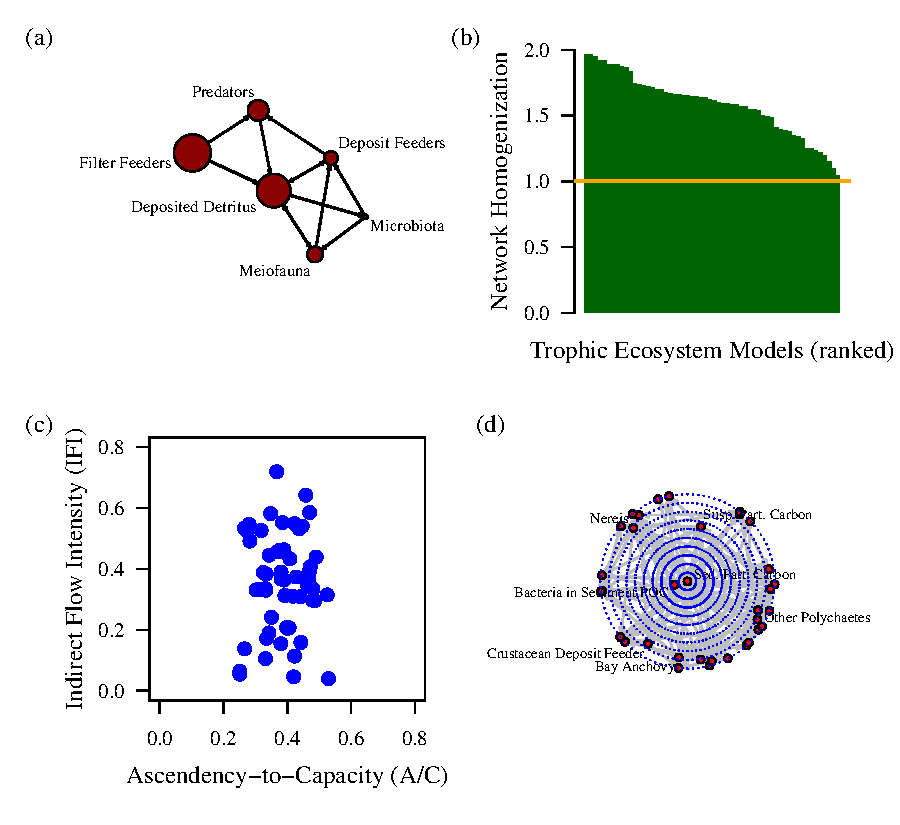
\includegraphics[scale=1]{../figures/enaR_plot_example.pdf}
\caption{Example of analysis and visualizations created with \enaR\:
  (a) network digraph of the internal flows of an oyster reef
  ecosystem model \citep{dame81}, (b) network homogenization statistic
  for 56 trophic ecosystem models (rank-ordered), (c) scatter plot
  showing the relationship between the ascendency-to-capacity ratio
  and the indirect flow index for the 56 trophic ecosystem models
  included in the package, and (d) target plot of the betweenness centrality from
  social network analysis calculated for the xx nodes of the
  Chesapeake Bay ecosystem model \citep{baird89}. } \label{fig:example}
\end{figure*}

\begin{figure*}[t]
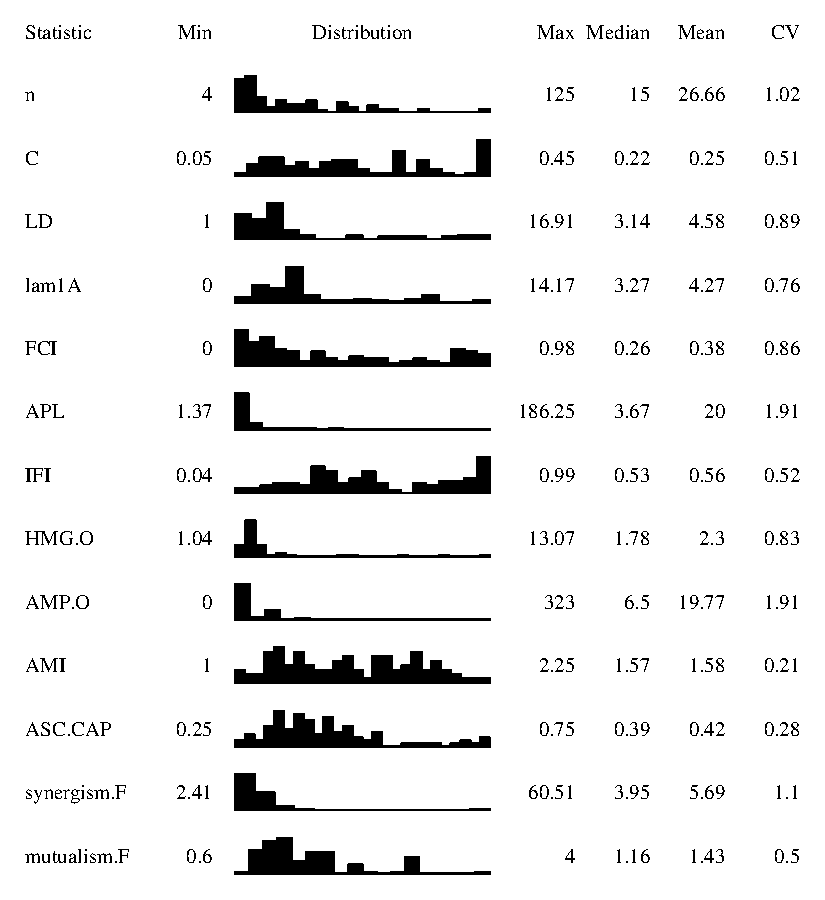
\includegraphics[scale=1]{../figures/ns_dist.pdf}
\caption{Distributions of selected ENA network statistics from the
  100 empirically-based ecosystem models included in \enaR.  The
  results are summarized using a histogram showing the distribution of
  the values of each network statistic between the observed minimum
  and maximum values.  The median, mean, and coefficient of variation
  (ratio of standard deviation and mean) values are also reported.
  The network statistics are the number of nodes ($n$), the
  connectance ($C = L/n^2$), link density ($LD = L/n$), pathway
  proliferation rate (lam1A), Finn cycling index (FCI), average path
  length (APL), indirect flow intensity (IFI), output oriented network
  homogenization ratio (HMG.O), output-oriented network amplification
  ratio (AMP.O), average mutual information (AMI), the
  ascendency-to-capacity ratio (ASC.CAP), flow-based network synergism
  (synergism.F) and mutualism (mutualism.F).} \label{fig:ns}
\end{figure*}

\end{document}
